\documentclass[letterpaper,12pt]{article}
\usepackage[utf8]{inputenc}
\usepackage{geometry}
\usepackage{amsmath}
\usepackage{float}
\usepackage{graphicx}
\usepackage{amssymb}
\usepackage{fancyhdr}

\title {\textbf{Cálculos en Multisim}}
\author{Lara Xocuis Martha Denisse}
\date{10 de abril, 2023}
\geometry{top=2cm, bottom=2cm, left=2cm, right= 2cm} %%margen
\graphicspath{{images/}}
\parindent=0pt

\begin{document}
\maketitle

\begin{sloppypar} 
\section{Circuito en serie}
\begin{figure}[H]
    \centering
    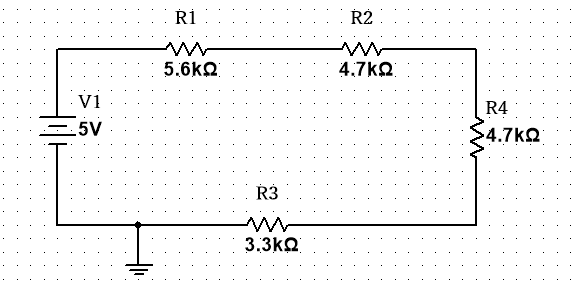
\includegraphics[width=0.6\textwidth]{images/proytec/cir.png}
    \caption{Circuito en serie a calcular y medir}
\end{figure}

\renewcommand{\theenumi}{\alph{enumi}}

\begin{enumerate}
    \item Medición de resistencia total por ohmetro
    \begin{figure}[H]
        \centering
        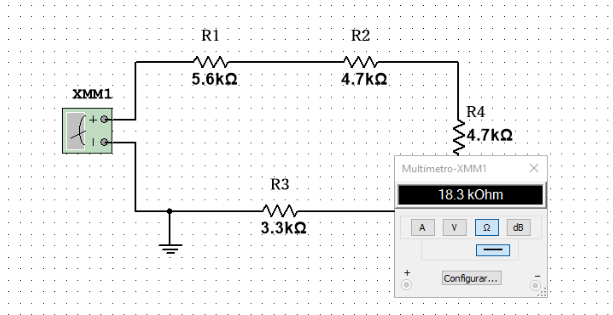
\includegraphics[width=0.7\textwidth]{images/proytec/srt.png}
    \end{figure}
\newpage
    \item Medición de voltaje total y parcial
    \begin{figure}[H]
        \centering
        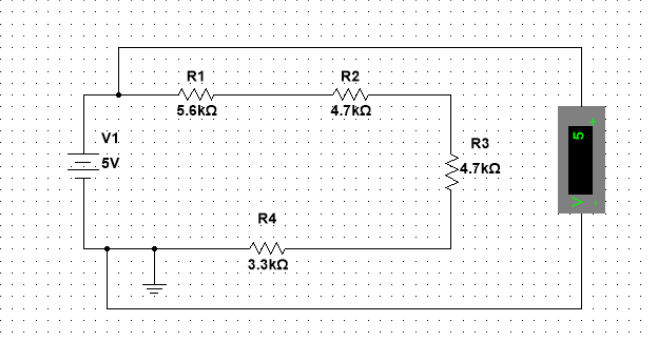
\includegraphics[width=0.7\textwidth]{images/proytec/svt.png}
        \caption{voltaje total por voltímetro}
    \end{figure}
    \begin{figure}[H]
        \centering
        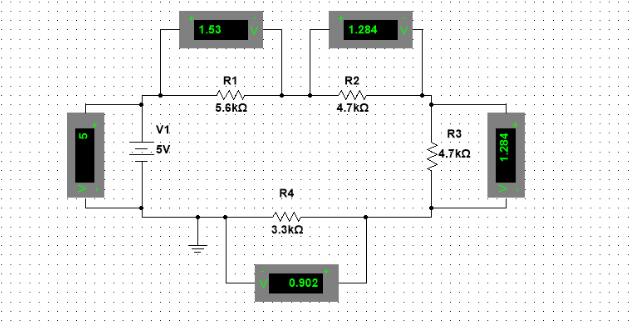
\includegraphics[width=0.7\textwidth]{images/proytec/svp.png}
        \caption{voltaje parcial por voltímetro}
    \end{figure}
    \item Medición de corriente de fuente a R1, R1 a R2, R2 a R3 y R4 a la fuente. 
    \begin{figure}[H]
        \centering
        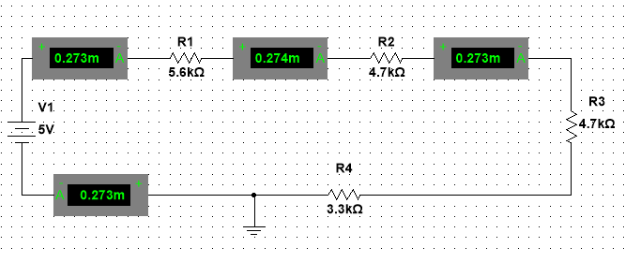
\includegraphics[width=0.6\textwidth]{images/proytec/sct.png}
    \end{figure}
\newpage
    \item Medición de potencia total y parcial por wattmetro
    \begin{figure}[H]
        \centering
        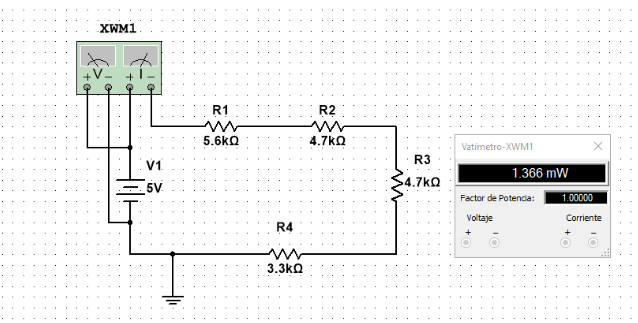
\includegraphics[width=0.7\textwidth]{images/proytec/spt.png}
        \caption{potencia total por wattmetro}
    \end{figure}
    \begin{figure}[H]
        \centering
        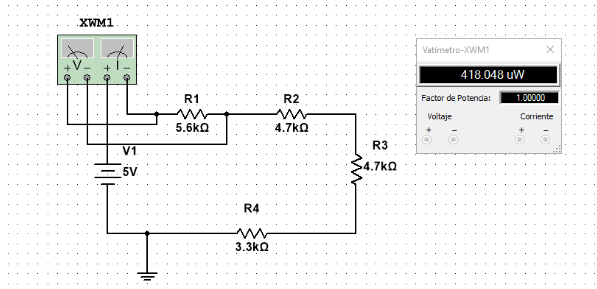
\includegraphics[width=0.6\textwidth]{images/proytec/sp1.png}
        \caption{potencia 1}
    \end{figure}
    \begin{figure}[H]
        \centering
        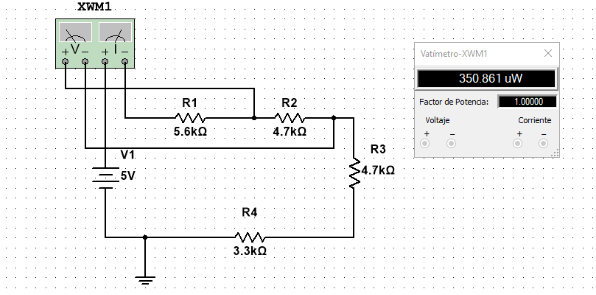
\includegraphics[width=0.6\textwidth]{images/proytec/sp2.png}
        \caption{potencia 2}
    \end{figure}
    \begin{figure}[H]
        \centering
        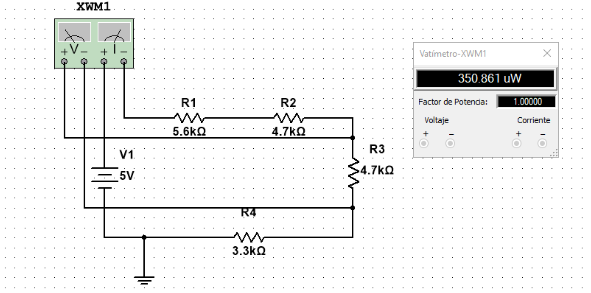
\includegraphics[width=0.6\textwidth]{images/proytec/sp3.png}
        \caption{potencia 3}
    \end{figure}
    \begin{figure}[H]
        \centering
        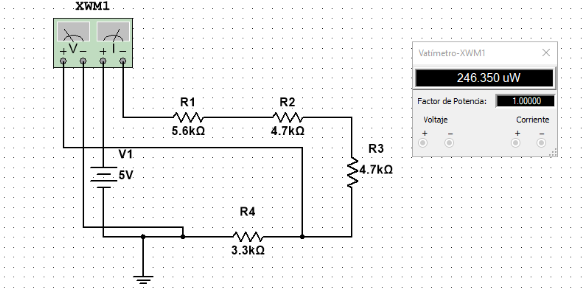
\includegraphics[width=0.6\textwidth]{images/proytec/sp4.png}
        \caption{potencia 4}
    \end{figure}
\newpage
    \item Medición de voltaje por osciloscopio 
    \begin{figure}[H]
        \centering
        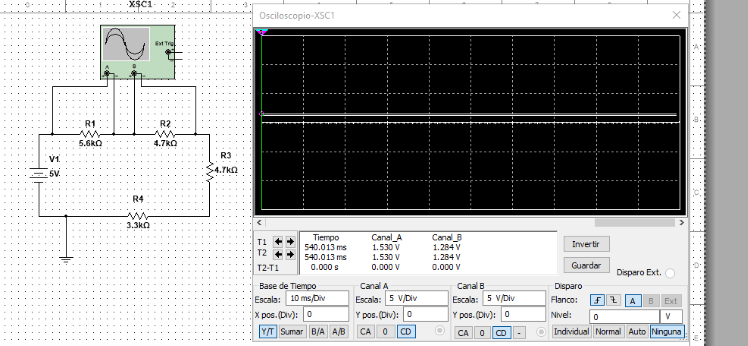
\includegraphics[width=0.7\textwidth]{images/proytec/svo1.png}
        \caption{Voltaje parcial en R1 y R2 por osciloscopio}
    \end{figure}
    \begin{figure}[H]
        \centering
        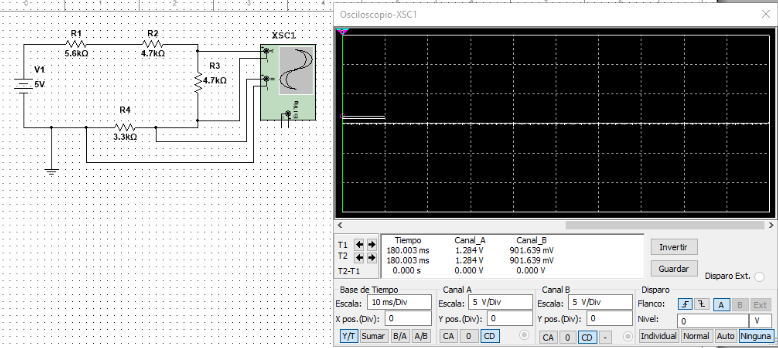
\includegraphics[width=0.7\textwidth]{images/proytec/svo2.png}
        \caption{Voltaje parcial en R3 y R4 por osciloscopio}
    \end{figure}
\end{enumerate}

\section{Circuito paralelo}
\begin{figure}[H]
    \centering
    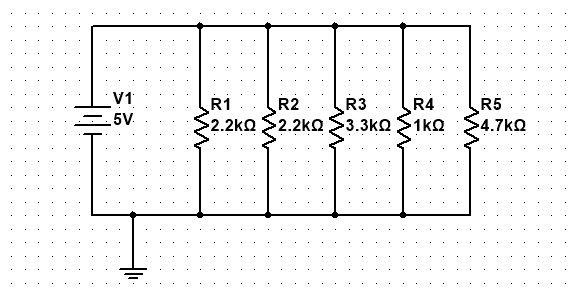
\includegraphics[width=0.6\textwidth]{images/proytec/cirp.png}
    \caption{Circuito en paralelo a calcular y medir}
\end{figure}
\begin{enumerate}
    \item Medición de resistencia total con ohmetro
    \begin{figure}[H]
        \centering
        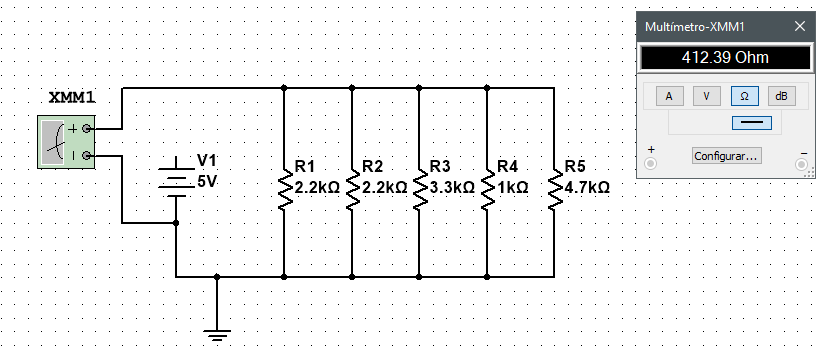
\includegraphics[width=0.7\textwidth]{images/proytec/prt.PNG}
    \end{figure}
    \item Conectando voltímetro en 3 lugares diferentes 
    \begin{figure}[H]
        \centering
        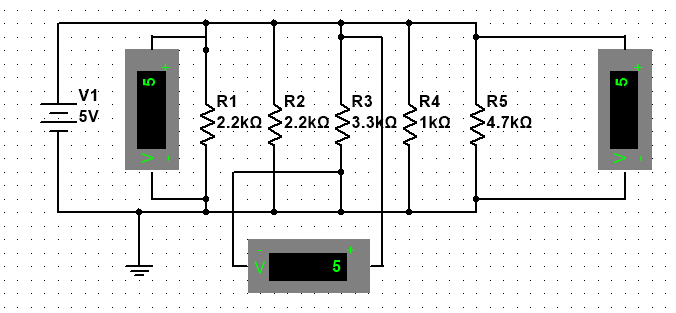
\includegraphics[width=0.6\textwidth]{images/proytec/pvt.PNG}
    \end{figure}
    \item Medición de corriente total y parcial con amperímetro 
    \begin{figure}[H]
        \centering
        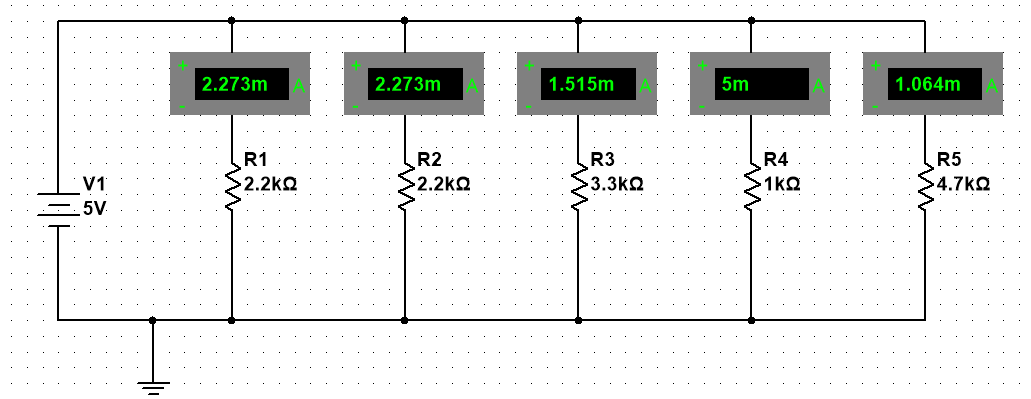
\includegraphics[width=0.7\textwidth]{images/proytec/pcp.PNG}
        \caption{corriente parcial con amperímetro}
    \end{figure}
\newpage
    \begin{figure}[H]
    \centering
    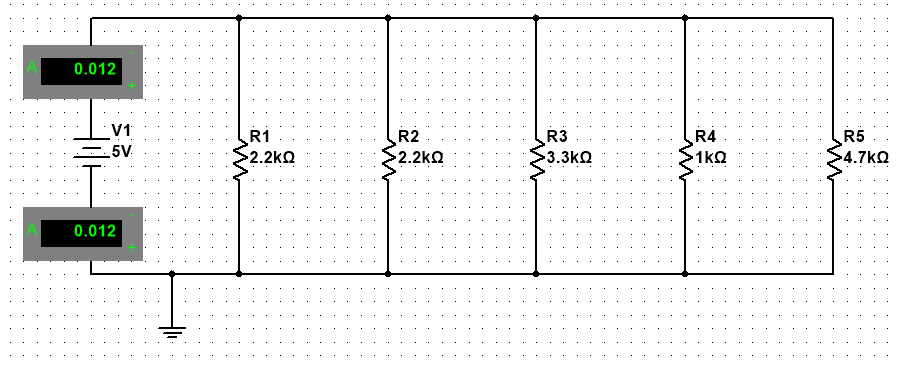
\includegraphics[width=0.7\textwidth]{images/proytec/pct2.PNG}
    \caption{corriente total con amperímetro}
    \end{figure}
    \item Medición de potencia total y parcial con wattmetro 
    \begin{figure}[H]
        \centering
        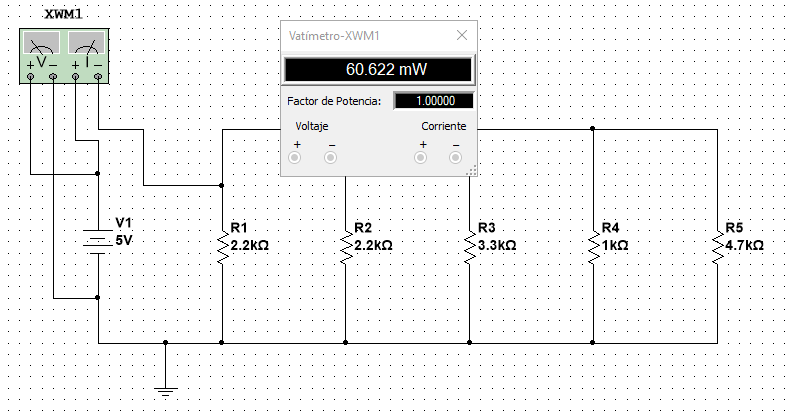
\includegraphics[width=0.7\textwidth]{images/proytec/ppt.PNG}
        \caption{potencia total con wattmetro}
    \end{figure}
    \begin{figure}[H]
        \centering
        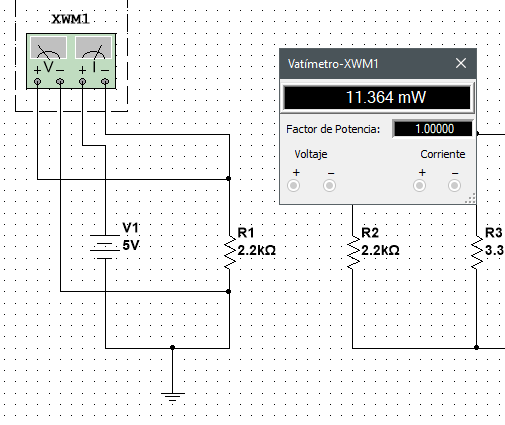
\includegraphics[width=0.6\textwidth]{images/proytec/pp1.png}
        \caption{potencia 1}
    \end{figure}
    \begin{figure}[H]
        \centering
        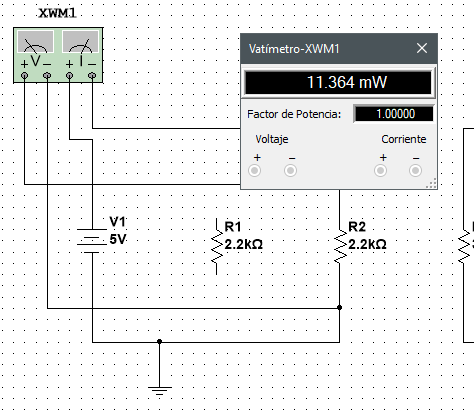
\includegraphics[width=0.6\textwidth]{images/proytec/pp2.PNG}
        \caption{potencia 2}
    \end{figure}
    \begin{figure}[H]
        \centering
        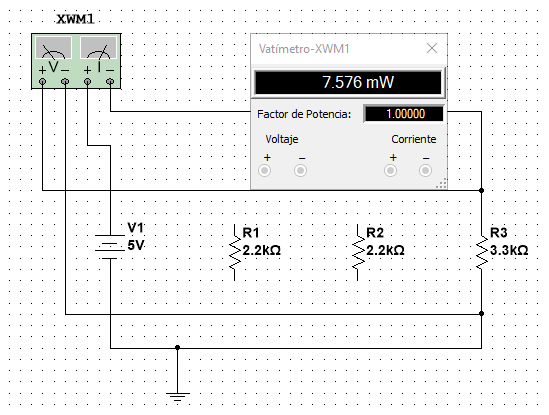
\includegraphics[width=0.7\textwidth]{images/proytec/pp3.png}
        \caption{potencia 3}
    \end{figure}
    \begin{figure}[H]
        \centering
        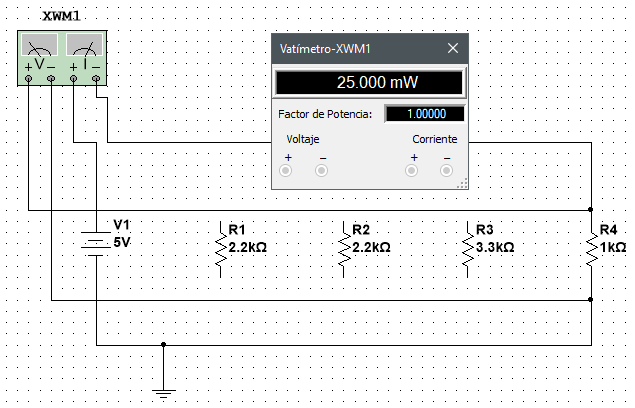
\includegraphics[width=0.7\textwidth]{images/proytec/pp4.png}
        \caption{potencia 4}
    \end{figure}
    \begin{figure}[H]
        \centering
        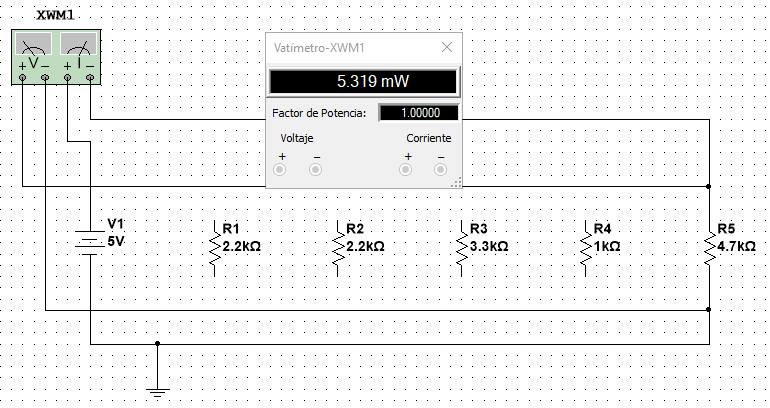
\includegraphics[width=0.7\textwidth]{images/proytec/pp5.png}
        \caption{potencia 5}
    \end{figure}
\end{enumerate}


\end{sloppypar}
\end{document}